\documentclass[10pt]{article}
\usepackage[final]{graphicx}
\usepackage{amsfonts}

\topmargin -.5in
\textwidth 6.6in
\textheight 9in
\oddsidemargin 0in
\usepackage{color}
\newcommand{\arvind}[1]{{\color{red}{Arvind: {#1}}}}

\def\ds{\displaystyle}
\def\d{\partial}
\linespread{1.5}

\begin{document}



%%%%%%%%%%%%% 
\section{Computational Experiments}
\arvind{I suggest organizing this section into a series of experiments. Here are a few suggestions. You can also follow the instructions at the end of the section.}

\subsection{Experiment 1: Analysis of PM25 time series}

\subsubsection{Holt-Winters Exponential Smoothing}
We firstly draw fitted value plot based on Holt-Winters Exponential Smoothing. In the plot below, black line represents the variation of real PM value during 2004-2014 and red line represents the variation of fitted PM value during the period. We can see that although the two lines have similar trend, the fitted value is not accurate enough at many points.

\begin{figure}[ht!]
\centering
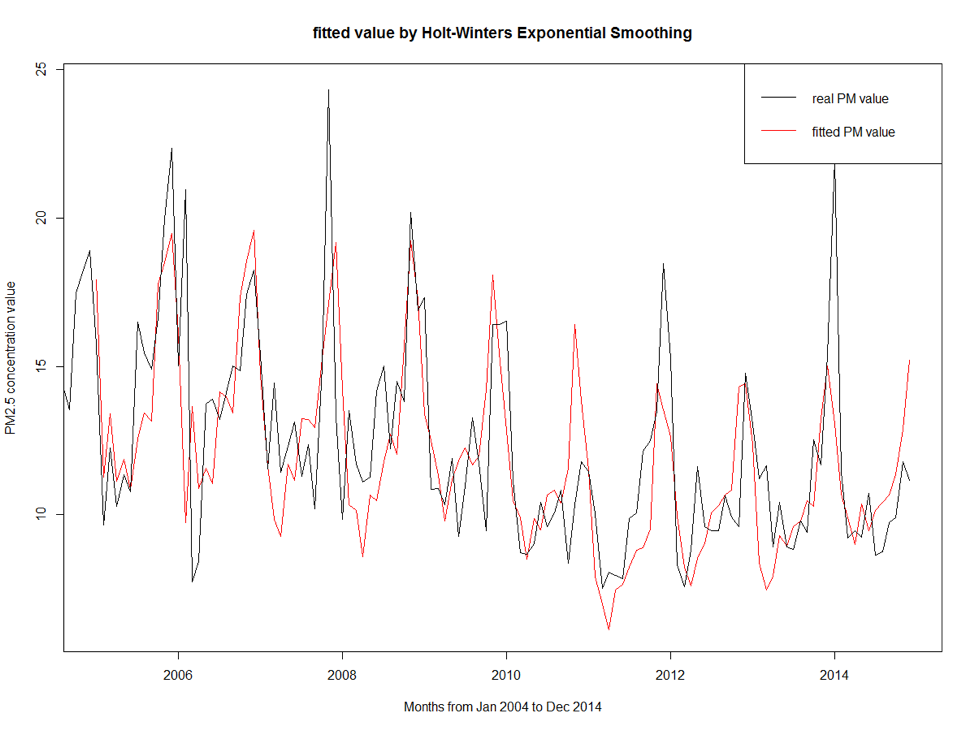
\includegraphics[width = 90mm]{ts2.png}
%\caption{}
%\label{graph4}
\end{figure}

Then we predict the PM2.5 concentration value for the whole year 2015. In the plot below, the blue line represents the predicted value for 2015. The shadow of deep color represents the 80\% prediction interval for the predicted value and the shadow of light color represents the 95\% prediction interval for the predicted value.

\begin{figure}[ht!]
\centering
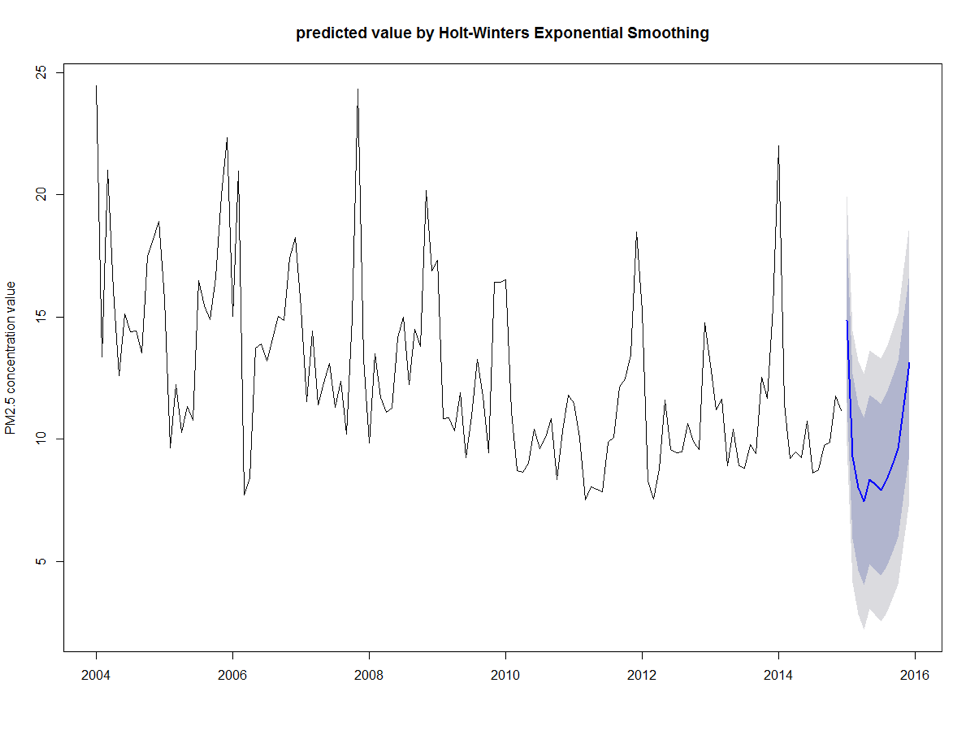
\includegraphics[width = 90mm]{ts3.png}
%\caption{}
%\label{graph4}
\end{figure}

Now let?u exmaine the effect of our prediction. We decide to use mean square error as our criterion. Lower mean square error indicates we have a better prediction. By comparing the predicted results and the real PM value for the year 2015, we find the mean square error between them is around 5.5. Becaues the mean of PM2.5 value during 2004-2014 is about 12.6, the mean square error is kind of large and this model is not very accurate.

\subsubsection{ARIMA model}
Becaues there seems to exist seasonality in the PM2.5 value time series, we want to decompose the time series and apply ARIMA model to the adjusted time series. We first decompose the PM2.5 concentration value time series and plot it. In the plot below, the four subplots respectively represent observed value, overall trend component, seasonal component and random part. From the seasonal component, we can see that there does exist differences of PM2.5 value among different months. By subtracting the seasonal component from the original time series, we get adjusted PM2.5 concentration value time series.

\begin{figure}[ht!]
\centering
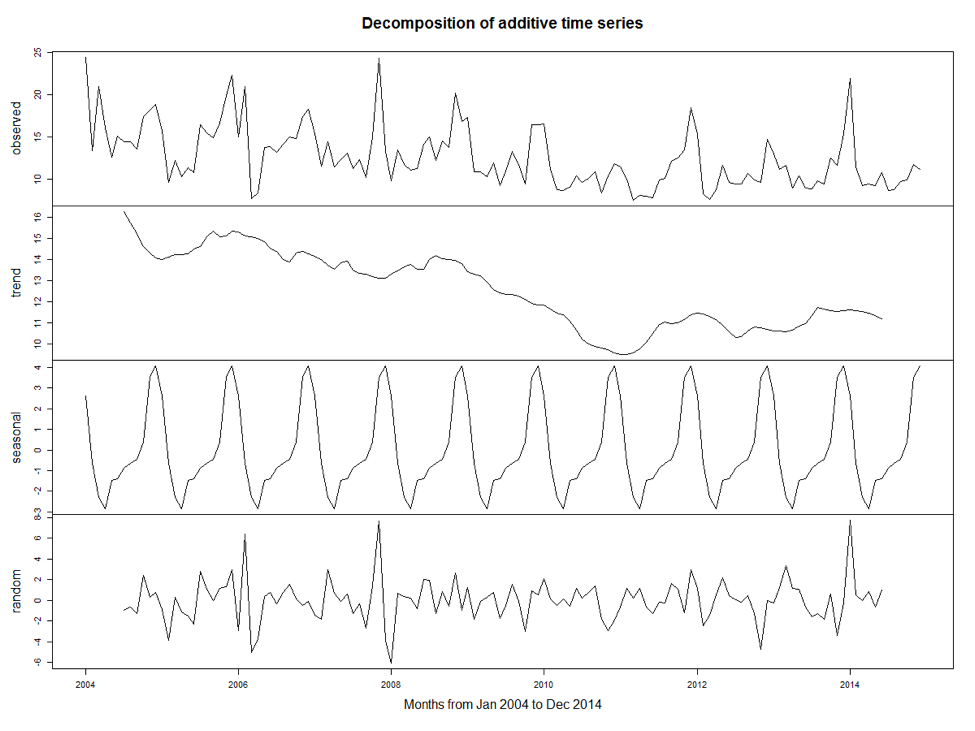
\includegraphics[width = 90mm]{ts4.png}
%\caption{}
%\label{graph4}
\end{figure}

Then we draw fitted adjusted PM value based on ARIMA model. The black line represents the variation of real adjusted PM value during 2004-2014 and red line represents the variation of fitted adjusted PM value during the period. From this plot we can see that the fitted line is really rough.

\begin{figure}[ht!]
\centering
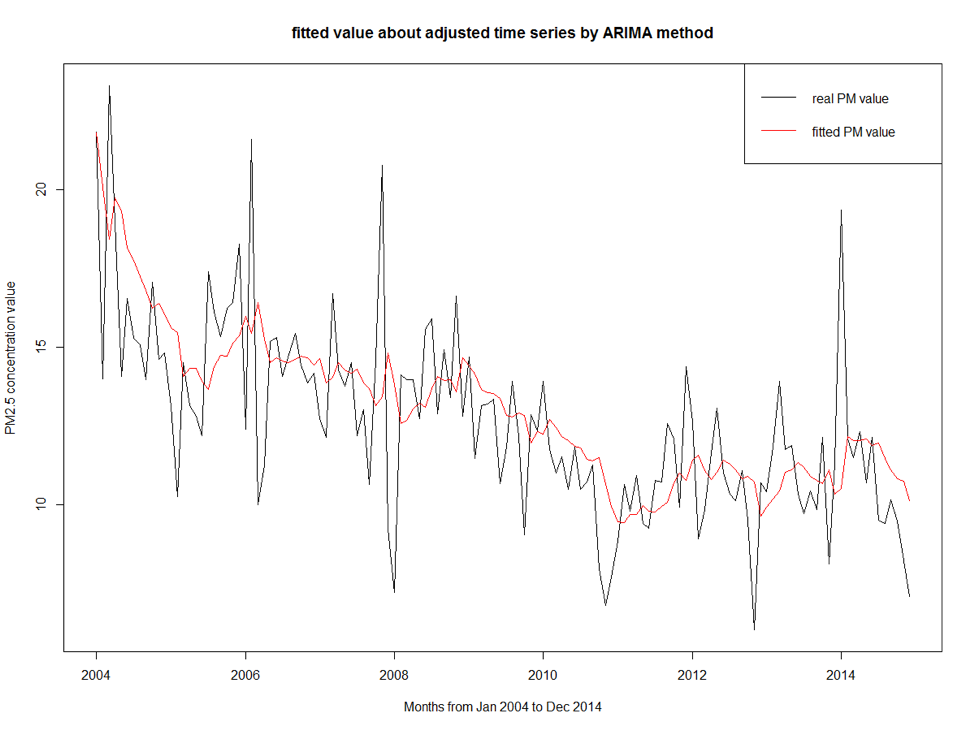
\includegraphics[width = 90mm]{ts5.png}
%\caption{}
%\label{graph4}
\end{figure}

Next, we predict the adjusted PM2.5 concentration value for the whole year 2015. Similar as before, , the blue line represents the predicted value for 2015. The shadow of deep color represents the 80\% prediction interval for the predicted value and the shadow of light color represents the 95\% prediction interval for the predicted value.

\begin{figure}[ht!]
\centering
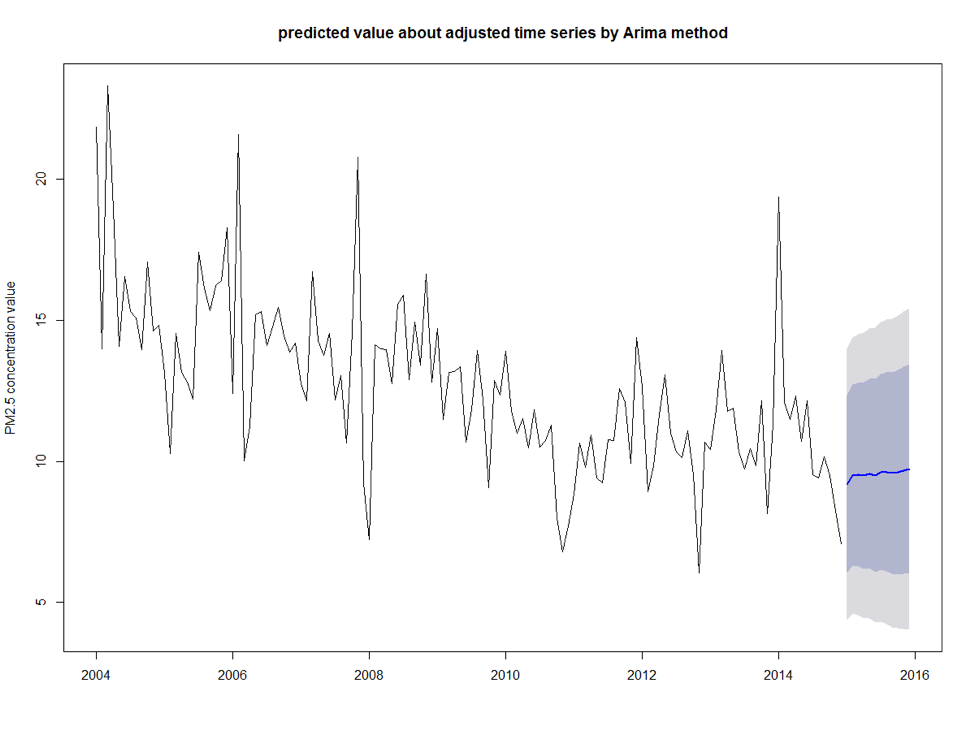
\includegraphics[width = 90mm]{ts6.png}
%\caption{}
%\label{graph4}
\end{figure}

Finally, we adding seasonal component to our predicted result and then compare it with the real PM value during 2004-2014. We find the mean square error is around 9.7. So the performance of ARIMA model is even not as good as Holt-Winters Exponential Smoothing.

In sum, the effect of prediction by time series is not very good. But it does give us some inspiration. For example, the PM 2.5 value will be different in different seasons. For next step

\subsection{Experiment 2: PM 25 vs AOT data}

\subsubsection{Sites closest to the west coast}
If we only use the AOD data, by using the approach in Section ????, we fitted the mixed effects model as follows.

$$\hat{PM}_{ij} = 10.51 + 3.60\times AOD_{ij} + \hat{s}_i + \hat{d}_j, $$

where $\hat{s}_i\sim N(0, 1.79^2)$ and $\hat{d}_j\sim N(0, 3.04^2)$. 

The correlation between the fitted PM$_{2.5}$ data and the true PM$_{2.5}$ data is 0.802, which we agreed it is not a bad fit. 

If we use both the AOD data and the wind data, we built a multivariate linear regression model. As in Figure XXX, different sites have different relationships between AOD and PM. 

The following analysis is about the site (40.80178, -124.1621). For other sites, analysis should be similar. 

$$\hat{PM} = -0.64 - 0.0176\times AOD - 0.11\times WindSpeed + 0.45\times WindDirection + 0.017\times Humidity - 0.16\times AirTemp + Season + Year, $$

where Season and Year are factor variables. $R^2 = 0.758$.

\begin{figure}[ht!]
\centering
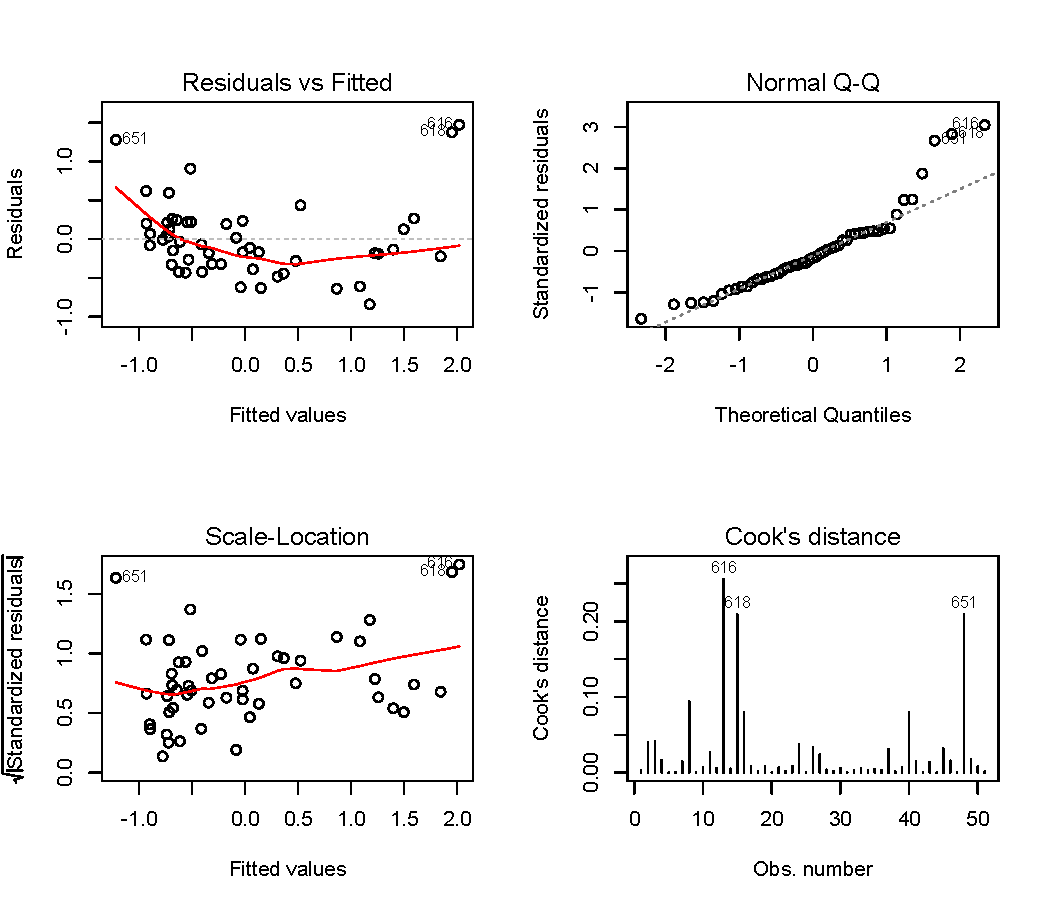
\includegraphics[width = 90mm]{residual.pdf}
\caption{}
\label{graph5}
\end{figure}

We can see from the above plots that there are three outliers. After deleting these outliers, the model became:

$$\hat{PM} = 94.43 + 2.34\times AOD - 1.11\times WindSpeed + 0.033\times WindDirection - 0.068\times Humidity - 0.30\times AirTemp + Season + Year, $$

where Season and Year are factor variables. $R^2 = 0.822$.

Then we did the stepwise to choose the best fit, we get the following model:

$$\hat{PM} = 3.42 -1.07\times WindSpeed + 0.036\times WindDirection + Season, $$
where Season is a factor variable. $R^2 = 0.786$.

\begin{figure}[ht!]
\centering
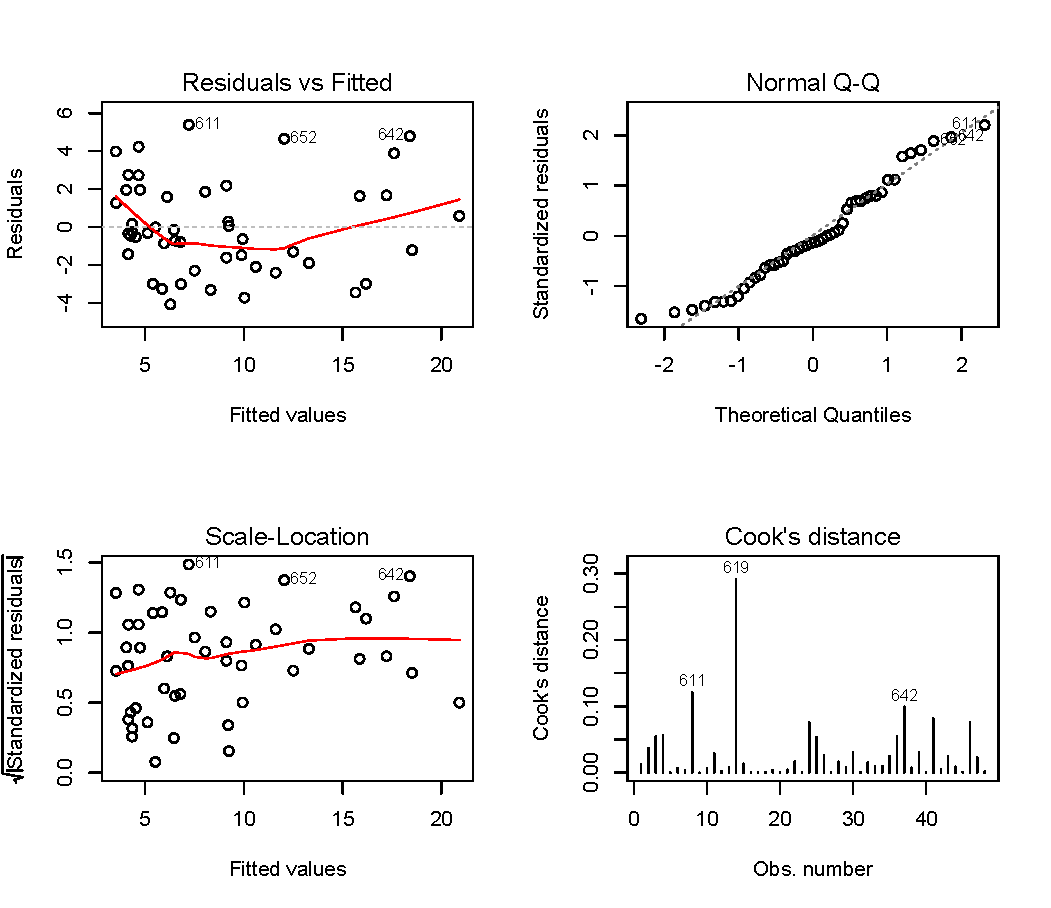
\includegraphics[width = 90mm]{residual2.pdf}
\caption{}
%\label{graph5}
\end{figure}

The results are better than the previous model. But we can see from those plots that the residuals still have some trend and some cluster. To figure out if this model is good, we did 5-folder cross validation. The results are as follows:

\begin{figure}[ht!]
\centering
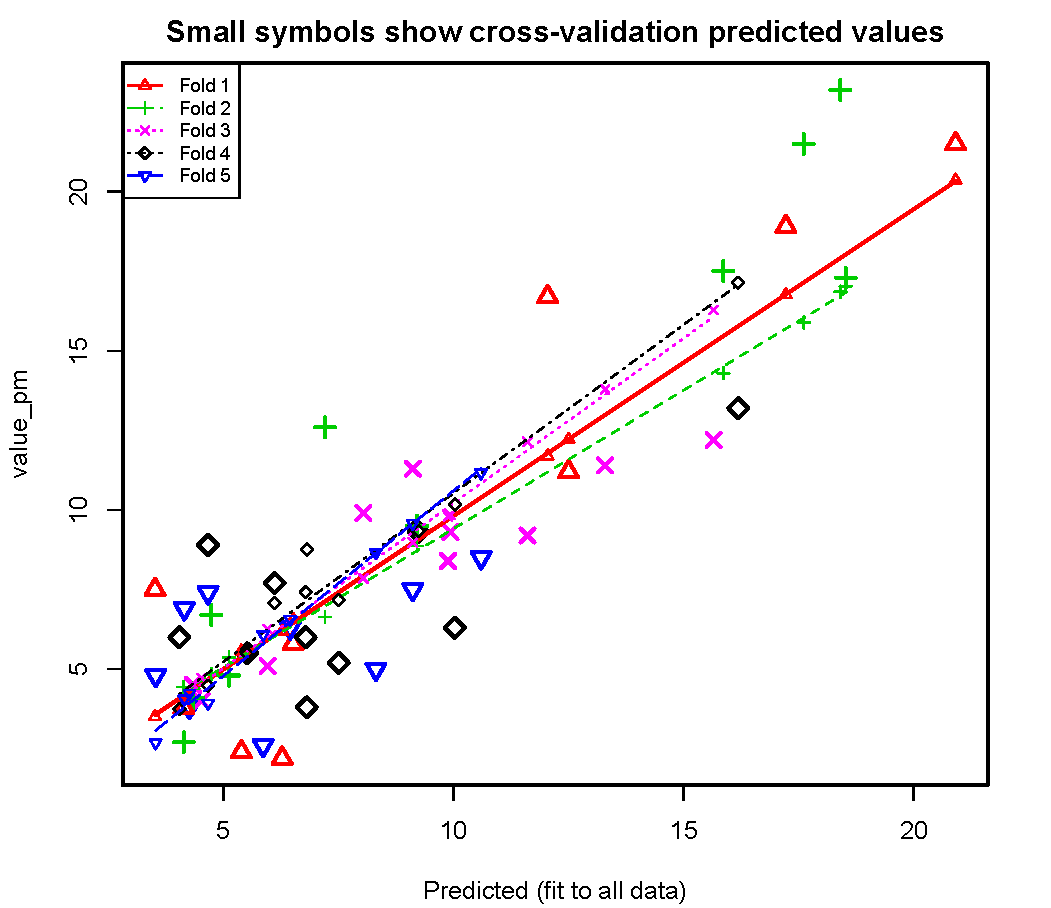
\includegraphics[width = 90mm]{cv_lm.pdf}
\caption{}
%\label{graph5}
\end{figure}

The mean square error is 8.16, which is very high due to the average PM values is 8.75. So multivariate linear regression is not a good model.

\subsubsection{Hawaii sites}
Similarly, we can get the mixed effects model for Hawaii sites.
Without the wind data,

$$\hat{PM}_{ij} = 6.205 + 7.780\times AOD_{ij} + \hat{s}_i + \hat{d}_j, $$

where $\hat{s}_i\sim N(0, 4.05^2)$ and $\hat{d}_j\sim N(0, 2.83^2)$. 

The correlation between the fitted PM$_{2.5}$ data and the true PM$_{2.5}$ data is 0.879, which is better than the west coast data. 


%\subsubsection{Only AOD data}
%Since there are many meteorological parameters varying from day to day, our statistical model must have the variability of the date. For each location, there are many different geographical properties, so our model must have the variability of sites. Therefore we used mixed effects model to fit this relationship:
%
%$$PM_{ij} = \alpha + \beta\times AOD_{ij} + s_i + d_j+ \epsilon_{ij}, $$
%
%where $PM_{ij}$ is the $PM_{2.5}$ concentration at a spatial site $i$ on a specific day $j$, $\alpha$ is the fixed intercept, $\beta$ is the fixed slope, $AOD_{ij}$ is the AOD value at a spatial site $i$ on a specific day $j$, $s_i\sim N(0, \sigma_s^2)$ is the random intercept of site $i$, $d_j\sim N(0, \sigma_d^2)$ is the random intercept of a specific day $j$, and $\epsilon_{ij}\sim N(0, \sigma^2)$ is the error term at site $i$ on a day $j$.
%
%\subsubsection{AOD data and wind data}
%


\subsubsection{relationships between AVHRR AOD and surface PM2.5 for sites closest to the west coast}

For sites closest to the west coast, we finally found 4 sites that have common date information. Figure \ref{fig3.3} is the plot regarding the AOD and PM2.5 by each site. 

\begin{figure}[!h]
\centering
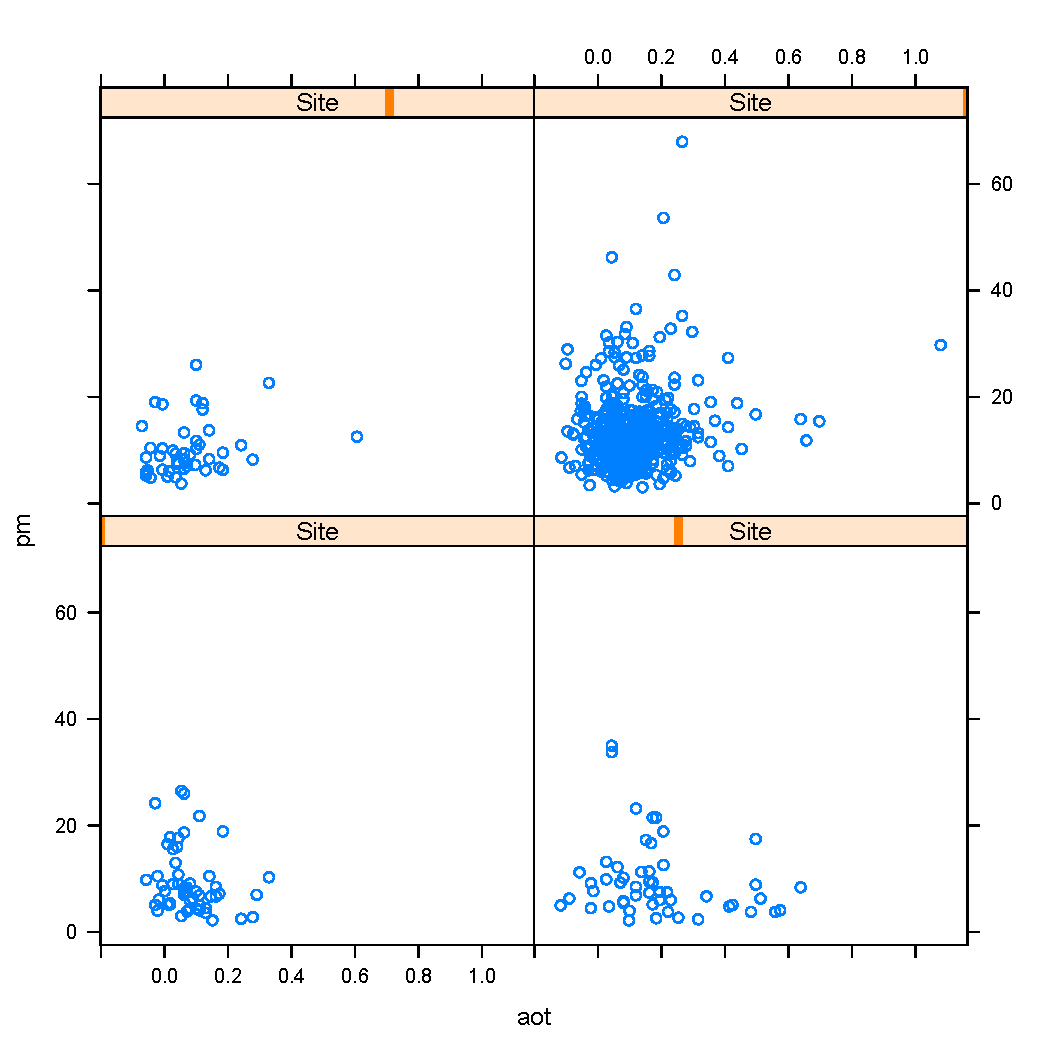
\includegraphics[width=\linewidth]{3.pdf}
\caption{PM vs. AOD for each site close to the west coast}
\label{fig3.3}
\end{figure}

We can see from the above plot that the relationships between AOD and PM2.5 are different for different sites. So we consider building different models for each site to find the relationships.

\subsubsection{relationships between AVHRR AOD and surface PM2.5 for Hawaii sites}

For Hawaii sites, we finally found 9 sites that have common date information. Figure \ref{fig3.4} is the plot regarding the AOD and PM2.5 by each site. 

\begin{figure}[!h]
\centering
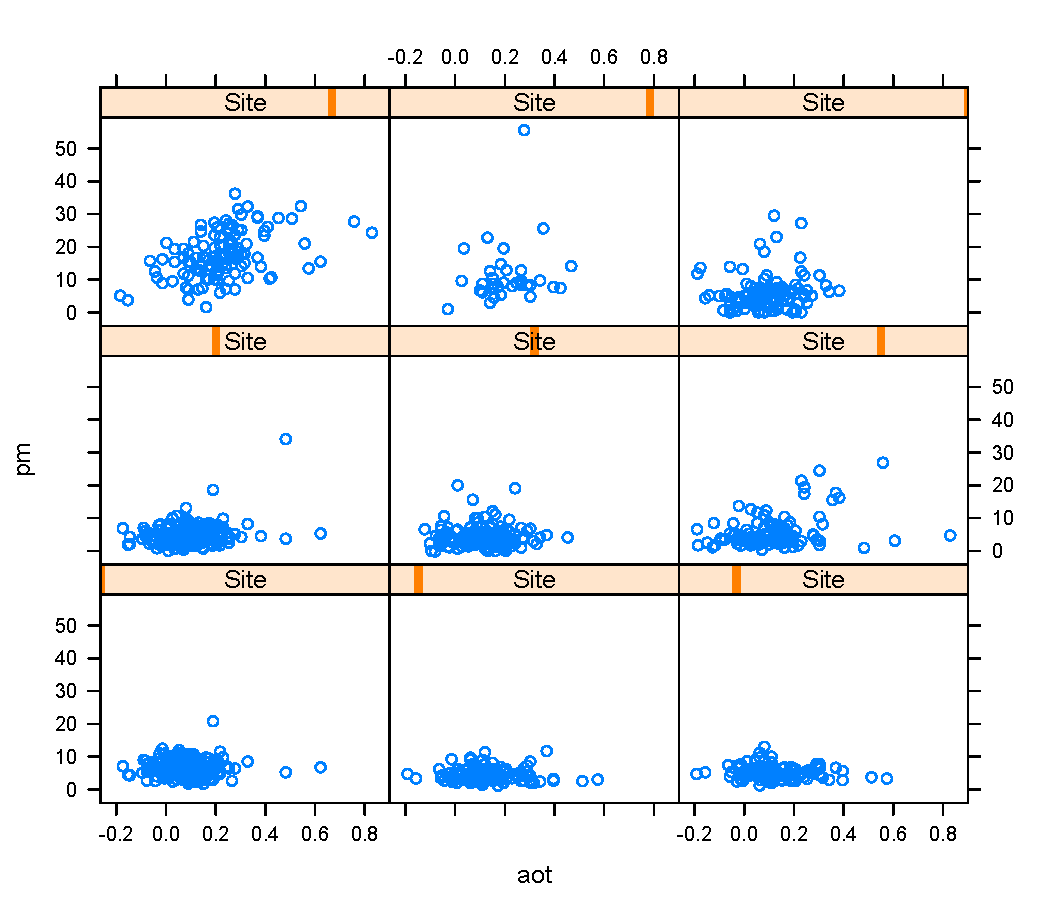
\includegraphics[width=\linewidth]{1.pdf}
\caption{PM vs. AOD for each Hawaii site}
\label{fig3.4}
\end{figure}

Similarly, we can see from the above plot that the relationships between AOD and PM2.5 are different for different sites. Like what we did for sites close to the west coast, we consider building different models for each site to find the relationships.
%%%%%%%%%%%%%%%%%%

%%%%%%%%%%%%%% This is NEHA's section
\subsection{Spatial Statistics}
We try to build spatial model for the AOT and PM data.In spatial statistics, we study the relations and variation in data with respect to its location. Spatial statistics on a geological data is carried out in two stages:

\begin{itemize}
\item Analyze the dataset to build a relatedness (covariance) amongst values based on their geographical location. In the language of statistics, this means building a variogram which models variance between values at two locations according to the distance and direction between them.
\item The next step is to estimates values at unsampled locations. This process is called "Kriging". The interpolated values are obtained by Kriging are modeled using a Gaussian process directed by prior covariances. In contrast, the focus while using polynomial interpolation is to optimize the smoothness of the interpolated values.
\end{itemize}

We use ordinary kriging to interpolate AOD and PM2.5 values.

In ordinary kriging, the interpolated value is a weighted linear combination of sampled values. Ordinary kriging assumes constant mean and  residual mean error to be 0. Along with this, ordinary kriging aims to minimize the variance of error. The variogram gives the covariances between different values. Ordinary kriging is obtained by using probability models that calculate the bias and error in variance, which can then be used to choose weights for neighbouring sampled locations such that mean error for the model is exactly zero and modelled error variance is minimized. We have used maximum likelihood probability model to estimate parameters. We obtain the spatial plots and standard error associated with  the interpolations using this method of kriging. 

There are 284 sensor sites that recorded the PM2.5 measurements. We use the daily  PM$_{2.5}$ measurements values at these sites to make spatial interpolation plots. Similarly, spatial interpolation plots are constructed for AOD values. 

%%%%%%%%%%%%%%%%%%%%%%%%%%

Give enough details so that readers can duplicate your experiments.

\begin{itemize}
\item Describe the precise purpose of the experiments, and what they 
are supposed to show.

\item Describe and justify your test data, and any assumptions you made to 
simplify the problem.

\item Describe the software you used, and the 
parameter values you selected.

\item 
For every figure, describe the meaning and units of the coordinate axes, 
and what is being plotted.

\item Describe the conclusions you can draw from your experiments
\end{itemize}

\end{document}